%========================================
% MatinBook - Stage 10: Graphics Test
% Test: TikZ + PGFPlots + Flowcharts + Trees + Statistical Charts
% Purpose: Validate all drawing and plotting capabilities
%========================================

\makeatletter
\def\input@path{{../}}
\makeatother

\documentclass{matinbook}

\title{آزمون سیستم گرافیک و نمودارها}
\author{تیم توسعه MatinBook}
\date{تابستان ۱۴۰۵}

\begin{document}

%----------------------------------------
% Title Page
%----------------------------------------
\maketitle

%----------------------------------------
% Chapter 1: Function Plots
%----------------------------------------
\chapter{نمودار توابع ریاضی}

\section{مقایسه توابع پایه}

\begin{figure}[h]
\centering
\begin{latin}
\begin{tikzpicture}
  \begin{axis}[
    width=14cm, height=8cm,
    xlabel={$x$},
    ylabel={$f(x)$},
    title={Comparison of Common Mathematical Functions},
    grid=major,
    legend pos=north west,
    domain=-3:3,
    samples=200,
    xmin=-3, xmax=3,
    ymin=-5, ymax=10
  ]
    % Quadratic function
    \addplot[matinblue, thick] {x^2};
    \addlegendentry{$x^2$}
    
    % Cubic function
    \addplot[matinred, thick] {x^3};
    \addlegendentry{$x^3$}
    
    % Exponential function
    \addplot[matinorange, thick] {exp(x)};
    \addlegendentry{$e^x$}
    
    % Square root (only for x >= 0)
    \addplot[matingreen, thick, domain=0:3] {sqrt(x)};
    \addlegendentry{$\sqrt{x}$}
  \end{axis}
\end{tikzpicture}
\end{latin}
\caption{مقایسه توابع $x^{2}$، $x^{3}$، $e^{x}$ و $\sqrt{x}$}
\label{fig:basic-functions}
\end{figure}

\section{توابع مثلثاتی}

\begin{figure}[h]
\centering
\begin{latin}
\begin{tikzpicture}
  \begin{axis}[
    width=14cm, height=7cm,
    xlabel={$x$},
    ylabel={$f(x)$},
    title={Trigonometric Functions},
    grid=major,
    legend pos=north west,
    domain=-2*pi:2*pi,
    samples=300,
    xtick={-2*pi, -1.5*pi, -pi, -0.5*pi, 0, 0.5*pi, pi, 1.5*pi, 2*pi},
    xticklabels={$-2\pi$, $-\frac{3\pi}{2}$, $-\pi$, $-\frac{\pi}{2}$, 
                 $0$, $\frac{\pi}{2}$, $\pi$, $\frac{3\pi}{2}$, $2\pi$},
    ymin=-1.5, ymax=1.5
  ]
    \addplot[matinblue, thick] {sin(deg(x))};
    \addlegendentry{$\sin x$}
    
    \addplot[matinred, thick] {cos(deg(x))};
    \addlegendentry{$\cos x$}
    
    \addplot[matinorange, thick, dashed, restrict y to domain=-3:3] {tan(deg(x))};
    \addlegendentry{$\tan x$}
  \end{axis}
\end{tikzpicture}
\end{latin}
\caption{توابع مثلثاتی $\sin x$، $\cos x$ و $\tan x$}
\label{fig:trig-functions}
\end{figure}

\section{نمودار چندگانه با محورهای مختلف}

\begin{figure}[h]
\centering
\begin{latin}
\begin{tikzpicture}
  \begin{axis}[
    width=14cm, height=7cm,
    xlabel={$x$},
    ylabel={$y$},
    title={Multiple Functions with Custom Styles},
    grid=major,
    legend pos=north west,
    domain=-5:5,
    samples=200
  ]
    % Sigmoid function
    \addplot[matinblue, ultra thick] {1/(1+exp(-x))};
    \addlegendentry{$\sigma(x) = \frac{1}{1+e^{-x}}$}
    
    % Hyperbolic tangent
    \addplot[matinpurple, thick, dashed] {tanh(x)};
    \addlegendentry{$\tanh x$}
    
    % ReLU approximation
    \addplot[matinorange, thick, dotted] {max(0, x)};
    \addlegendentry{$\max(0, x)$}
  \end{axis}
\end{tikzpicture}
\end{latin}
\caption{توابع فعال‌سازی در شبکه‌های عصبی}
\label{fig:activation-functions}
\end{figure}

\clearpage

%----------------------------------------
% Chapter 2: Statistical Charts
%----------------------------------------
\chapter{نمودارهای آماری}

\section{نمودار میله‌ای}

\begin{figure}[h]
\centering
\begin{latin}
\begin{tikzpicture}
  \begin{axis}[
    width=14cm, height=7cm,
    ybar,
    symbolic x coords={Python, JavaScript, Java, C++, Go, Rust, TypeScript},
    xtick=data,
    ylabel={محبوبیت (\%)},
    title={Programming Language Popularity - 2025},
    grid=major,
    bar width=18pt,
    ymin=0, ymax=35,
    nodes near coords,
    nodes near coords align={vertical},
    every node near coord/.append style={font=\small}
  ]
    \addplot[fill=matinblue!70] coordinates {
      (Python, 30)
      (JavaScript, 24)
      (Java, 17)
      (C++, 12)
      (Go, 8)
      (Rust, 5)
      (TypeScript, 4)
    };
  \end{axis}
\end{tikzpicture}
\end{latin}
\caption{محبوبیت زبان‌های برنامه‌نویسی در سال ۲۰۲۵}
\label{fig:language-popularity}
\end{figure}

\section{نمودار خطی مقایسه‌ای}

\begin{figure}[h]
\centering
\begin{latin}
\begin{tikzpicture}
  \begin{axis}[
    width=14cm, height=7cm,
    xlabel={Input Size ($n$)},
    ylabel={Operations},
    title={Algorithm Complexity Comparison},
    grid=major,
    legend pos=north west,
    domain=0:50,
    samples=100,
    ymin=0, ymax=3000
  ]
    % O(n^2)
    \addplot[matinred, thick] {x^2};
    \addlegendentry{$O(n^2)$}
    
    % O(n log n)
    \addplot[matinorange, thick] {x*ln(x)};
    \addlegendentry{$O(n \log n)$}
    
    % O(n)
    \addplot[matinblue, thick] {x};
    \addlegendentry{$O(n)$}
    
    % O(log n)
    \addplot[matingreen, thick] {10*ln(x)};
    \addlegendentry{$O(\log n)$}
  \end{axis}
\end{tikzpicture}
\end{latin}
\caption{مقایسه رشد پیچیدگی الگوریتم‌ها}
\label{fig:complexity-comparison}
\end{figure}

\section{نمودار پراکندگی}

\begin{figure}[h]
\centering
\begin{latin}
\begin{tikzpicture}
  \begin{axis}[
    width=12cm, height=7cm,
    xlabel={Hours Studied},
    ylabel={Exam Score},
    title={Study Time vs. Exam Performance},
    grid=major,
    legend pos=south east
  ]
    % Scatter points
    \addplot[only marks, mark=*, color=matinblue, mark size=2pt] coordinates {
      (1, 45) (2, 52) (3, 58) (4, 65) (5, 70)
      (6, 75) (7, 80) (8, 85) (9, 88) (10, 92)
      (1.5, 48) (2.5, 55) (3.5, 62) (4.5, 68) (5.5, 73)
      (6.5, 78) (7.5, 82) (8.5, 86) (9.5, 90)
    };
    \addlegendentry{Data points}
    
    % Regression line
    \addplot[matinred, thick, domain=0:11] {5*x + 40};
    \addlegendentry{Regression line}
  \end{axis}
\end{tikzpicture}
\end{latin}
\caption{نمودار پراکندگی با خط رگرسیون}
\label{fig:scatter-plot}
\end{figure}

\clearpage

%----------------------------------------
% Chapter 3: Flowcharts
%----------------------------------------
\chapter{فلوچارت‌ها و دیاگرام‌ها}

\section{فلوچارت تصمیم‌گیری}

\begin{figure}[h]
\centering
\begin{latin}
\begin{tikzpicture}[
  node distance=2cm,
  arrow/.style={thick,->,>=stealth}
]
  % Define nodes
  \node[block] (start) {Start};
  \node[block, below of=start] (input) {Read Input Data};
  \node[decision, below of=input] (validate) {Data Valid?};
  \node[block, right of=validate, xshift=3.5cm] (process) {Process Data};
  \node[block, below of=validate, yshift=-1.5cm] (error) {Show Error Message};
  \node[block, below of=process] (output) {Generate Output};
  \node[block, below of=output] (save) {Save Results};
  \node[block, below of=save] (end) {End};
  
  % Draw connections
  \draw[arrow] (start) -- (input);
  \draw[arrow] (input) -- (validate);
  \draw[arrow] (validate) -- node[anchor=south] {Yes} (process);
  \draw[arrow] (validate) -- node[anchor=east] {No} (error);
  \draw[arrow] (process) -- (output);
  \draw[arrow] (output) -- (save);
  \draw[arrow] (save) -- (end);
  \draw[arrow] (error) -- ++(-3.5,0) |- (input);
\end{tikzpicture}
\end{latin}
\caption{فلوچارت اعتبارسنجی و پردازش داده}
\label{fig:flowchart}
\end{figure}

\section{دیاگرام معماری نرم‌افزار}

\begin{figure}[h]
\centering
\begin{latin}
\begin{tikzpicture}[
  node distance=2.5cm,
  arrow/.style={thick,<->,>=stealth},
  component/.style={rectangle, draw=matindarkblue, fill=matinlightblue!30,
                    text width=3.5cm, text centered, rounded corners,
                    minimum height=2cm, font=\small}
]
  % Define components
  \node[component] (frontend) {Frontend\\React / Vue};
  \node[component, right of=frontend, xshift=3cm] (api) {REST API\\Express / FastAPI};
  \node[component, right of=api, xshift=3cm] (database) {Database\\PostgreSQL};
  
  \node[component, below of=api, yshift=-1.5cm] (cache) {Cache\\Redis};
  \node[component, left of=cache, xshift=-1.5cm] (queue) {Queue\\RabbitMQ};
  \node[component, right of=cache, xshift=1.5cm] (storage) {Storage\\S3 / MinIO};
  
  % Draw connections
  \draw[arrow] (frontend) -- (api);
  \draw[arrow] (api) -- (database);
  \draw[arrow] (api) -- (cache);
  \draw[arrow] (api) -- (queue);
  \draw[arrow] (api) -- (storage);
\end{tikzpicture}
\end{latin}
\caption{معماری یک برنامه وب مدرن}
\label{fig:architecture}
\end{figure}

\clearpage

%----------------------------------------
% Chapter 4: Trees and Graphs
%----------------------------------------
\chapter{درخت‌ها و گراف‌ها}

\section{درخت جستجوی دودویی (\lr{BST})}

\begin{figure}[h]
\centering
\begin{latin}
\begin{tikzpicture}[
  level distance=2cm,
  level 1/.style={sibling distance=5cm},
  level 2/.style={sibling distance=2.5cm},
  level 3/.style={sibling distance=1.5cm}
]
  \node[treenode] {50}
    child {node[treenode] {30}
      child {node[treenode] {20}}
      child {node[treenode] {40}
        child {node[treenode] {35}}
        child {node[treenode] {45}}
      }
    }
    child {node[treenode] {70}
      child {node[treenode] {60}}
      child {node[treenode] {80}
        child {node[treenode] {75}}
        child[missing]
      }
    };
\end{tikzpicture}
\end{latin}
\caption{درخت جستجوی دودویی (\lr{Binary Search Tree})}
\label{fig:bst}
\end{figure}

\section{درخت بیان ریاضی}

\begin{figure}[h]
\centering
\begin{latin}
\begin{tikzpicture}[
  level distance=1.8cm,
  level 1/.style={sibling distance=4cm},
  level 2/.style={sibling distance=2cm},
  opnode/.style={circle, draw=matinorange, fill=matinlightorange!30, minimum size=0.8cm},
  numnode/.style={circle, draw=matinblue, fill=matinlightblue!30, minimum size=0.8cm}
]
  \node[opnode] {$+$}
    child {node[opnode] {$\times$}
      child {node[numnode] {$3$}}
      child {node[numnode] {$x$}}
    }
    child {node[opnode] {$-$}
      child {node[numnode] {$5$}}
      child {node[numnode] {$2$}}
    };
\end{tikzpicture}
\end{latin}
\caption{درخت بیان ریاضی $3x + (5 - 2)$}
\label{fig:expression-tree}
\end{figure}

\section{گراف جهت‌دار}

\begin{figure}[h]
\centering
\begin{latin}
\begin{tikzpicture}[
  node distance=2.5cm,
  vertex/.style={circle, draw=matindarkblue, fill=matinlightblue!30,
                 minimum size=1cm, font=\bfseries},
  edge/.style={thick,->,>=stealth}
]
  % Define vertices
  \node[vertex] (A) at (0,0) {A};
  \node[vertex] (B) at (3,2) {B};
  \node[vertex] (C) at (6,0) {C};
  \node[vertex] (D) at (3,-2) {D};
  \node[vertex] (E) at (1.5,-3.5) {E};
  
  % Draw edges with weights
  \draw[edge] (A) -- node[anchor=south] {5} (B);
  \draw[edge] (B) -- node[anchor=south] {3} (C);
  \draw[edge] (C) -- node[anchor=west] {4} (D);
  \draw[edge] (D) -- node[anchor=north] {2} (A);
  \draw[edge] (A) -- node[anchor=east] {7} (E);
  \draw[edge] (D) -- node[anchor=east] {6} (E);
  \draw[edge] (B) to[bend left] node[anchor=west] {8} (D);
\end{tikzpicture}
\end{latin}
\caption{گراف وزن‌دار جهت‌دار با ۵ رأس}
\label{fig:directed-graph}
\end{figure}

\clearpage

%----------------------------------------
% Chapter 5: Advanced TikZ
%----------------------------------------
\chapter{نمودارهای پیشرفته}

\section{نمودار تابع سه‌بعدی}

\begin{figure}[h]
\centering
\begin{latin}
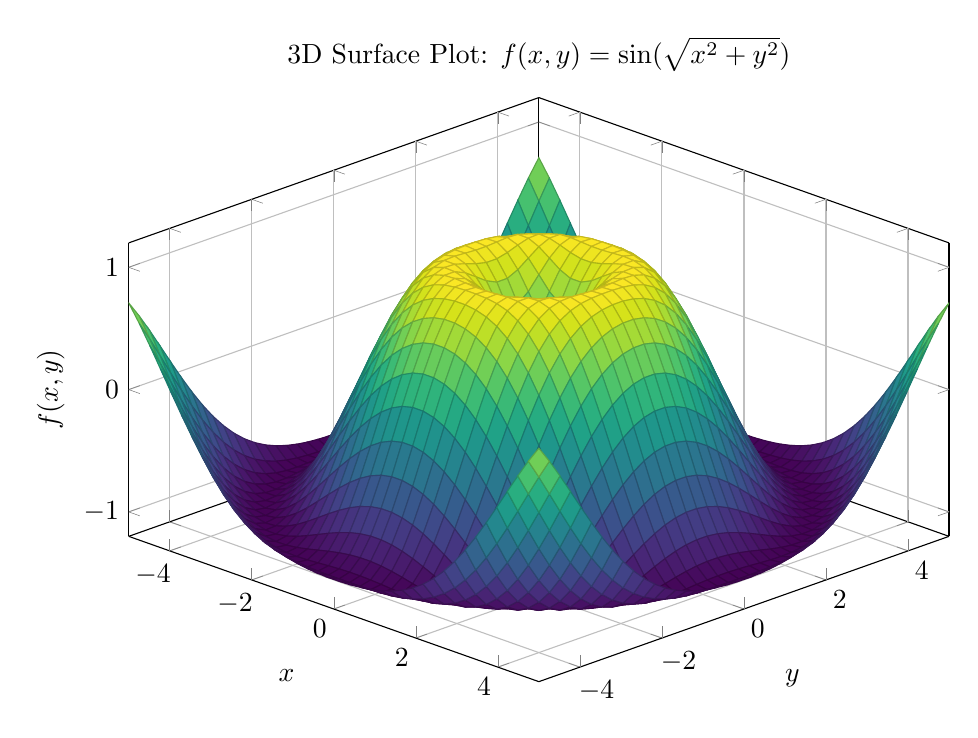
\begin{tikzpicture}
  \begin{axis}[
    width=12cm, height=9cm,
    xlabel={$x$},
    ylabel={$y$},
    zlabel={$f(x,y)$},
    title={3D Surface Plot: $f(x,y) = \sin(\sqrt{x^2+y^2})$},
    view={45}{35},
    grid=major
  ]
    \addplot3[
      surf,
      domain=-5:5,
      domain y=-5:5,
      samples=40,
      samples y=40,
      colormap/viridis
    ] {sin(deg(sqrt(x^2+y^2)))};
  \end{axis}
\end{tikzpicture}
\end{latin}
\caption{نمودار سه‌بعدی تابع $f(x,y) = \sin(\sqrt{x^{2}+y^{2}})$}
\label{fig:3d-surface}
\end{figure}

\section{نمودار دایره‌ای (\lr{Pie Chart})}

\begin{figure}[h]
\centering
\begin{latin}
\begin{tikzpicture}
  % Define colors for slices
  \definecolor{slice1}{RGB}{41, 128, 185}
  \definecolor{slice2}{RGB}{39, 174, 96}
  \definecolor{slice3}{RGB}{230, 126, 34}
  \definecolor{slice4}{RGB}{231, 76, 60}
  \definecolor{slice5}{RGB}{142, 68, 173}
  
  % Draw pie chart
  \pie[
    radius=3.5,
    text=legend,
    color={slice1, slice2, slice3, slice4, slice5}
  ]{
    35/Python,
    25/JavaScript,
    20/Java,
    12/C++,
    8/Other
  }
\end{tikzpicture}
\end{latin}
\caption{توزیع استفاده از زبان‌های برنامه‌نویسی}
\label{fig:pie-chart}
\end{figure}

\section{خط زمانی (\lr{Timeline})}

\begin{figure}[h]
\centering
\begin{latin}
\begin{tikzpicture}[
  timeline/.style={thick,->,>=stealth},
  event/.style={rectangle, draw=matindarkblue, fill=matinlightblue!30,
                text width=3.5cm, text centered, rounded corners,
                minimum height=1.5cm, font=\small}
]
  % Draw main timeline
  \draw[timeline] (0,0) -- (14,0);
  
  % Add year markers
  \foreach \x/\year in {0/1990, 3.5/2000, 7/2010, 10.5/2020, 14/2025} {
    \draw[thick] (\x,-0.2) -- (\x,0.2);
    \node[below] at (\x,-0.3) {\small\year};
  }
  
  % Add events
  \node[event, above] at (0,1.5) {Python\\Created};
  \node[event, above] at (3.5,1.5) {C\#\\Released};
  \node[event, above] at (7,1.5) {Rust\\First Stable};
  \node[event, below] at (7,-1.5) {Go\\Released};
  \node[event, above] at (10.5,1.5) {TypeScript\\Released};
  \node[event, below] at (14,-1.5) {AI/ML\\Boom};
  
  % Draw connections
  \draw[arrow] (0,0.3) -- (0,0.7);
  \draw[arrow] (3.5,0.3) -- (3.5,0.7);
  \draw[arrow] (7,0.3) -- (7,0.7);
  \draw[arrow] (7,-0.3) -- (7,-0.7);
  \draw[arrow] (10.5,0.3) -- (10.5,0.7);
  \draw[arrow] (14,-0.3) -- (14,-0.7);
\end{tikzpicture}
\end{latin}
\caption{خط زمانی تاریخچه زبان‌های برنامه‌نویسی}
\label{fig:timeline}
\end{figure}

%----------------------------------------
% Summary
%----------------------------------------
\chapter{خلاصه نتایج}

\section{وضعیت سیستم گرافیک}

\begin{table}[h]
\centering
\caption{وضعیت قابلیت‌های گرافیکی}
\label{tab:graphics-status}
\begin{tabular}{|c|C{6cm}|c|}
\hline
\textbf{نوع نمودار} & \textbf{موارد آزمایش شده} & \textbf{وضعیت} \\
\hline
توابع ریاضی & ۳ نمودار (پایه، مثلثاتی، فعال‌سازی) & \textcolor{matingreen}{✅} \\
نمودار آماری & میله‌ای، خطی، پراکندگی & \textcolor{matingreen}{✅} \\
فلوچارت & اعتبارسنجی داده + معماری نرم‌افزار & \textcolor{matingreen}{✅} \\
درخت & \lr{BST} + درخت بیان ریاضی & \textcolor{matingreen}{✅} \\
گراف & گراف وزن‌دار جهت‌دار & \textcolor{matingreen}{✅} \\
سه‌بعدی & نمودار سطح \lr{3D} & \textcolor{matingreen}{✅} \\
دایره‌ای & نمودار \lr{Pie Chart} & \textcolor{matingreen}{✅} \\
خط زمانی & تاریخچه زبان‌های برنامه‌نویسی & \textcolor{matingreen}{✅} \\
\hline
\end{tabular}
\end{table}

\section{نتیجه}

\textbf{ماژول گرافیک \lr{MatinBook} نسخه ۱ با موفقیت آزمایش شد.}
۱۲ نمودار مختلف شامل توابع ریاضی، نمودارهای آماری،
فلوچارت، درخت، گراف، نمودار سه‌بعدی و خط زمانی
به درستی رسم می‌شوند. 🎉

\end{document}